\documentclass[conference,a4paper]{IEEEtran}
\usepackage{amsmath,amssymb,mathtools}
\usepackage{booktabs}
\usepackage{siunitx}
\sisetup{detect-all, per-mode=symbol}
\DeclareSIUnit{\plato}{\textdegree P}
\DeclareSIUnit{\barg}{bar}
\usepackage{tikz}
\usetikzlibrary{arrows.meta,positioning}
\usepackage{cite}

\newcommand{\degP}{^{\circ}\mathrm{P}}

\title{Research for Solving Loss of Valve Authority and Analyser Delay in High-Gravity Beer Blending by Using Coordinated Delay-Compensated Active Disturbance Rejection Control}

\author{%
\IEEEauthorblockN{Thesis draft}%
\IEEEauthorblockA{Automatic control, 2026}%
}

\begin{document}
\maketitle

\begin{abstract}
Two limits remain after the inlet valves of a high-gravity blender have been given the correct flow gain. If the blend-header pressure is held at its design value while the beer supply falls, the beer valve runs out of stroke and the production rate is lost. If the original-extract loop is closed on the analyser, a transport delay of about ten seconds forces the loop to be slower than the brand changes it is asked to follow. This paper uses the outlet valve to track a header-pressure setpoint that keeps the three stems near their design openings, and it closes the extract loop on a mass-balance soft sensor whose bias is corrected by the delayed analyser. The bias update must subtract the bias itself. Without that subtraction a transient freezes as a permanent offset. On a \SI{560}{s} campaign the coordinated controller holds the beer flow through a rise to \SI{9}{\cubic\metre\per\hour} at a reduced supply, with stems near $0.70$, where both fixed-header baselines sit on the open stop.
\end{abstract}

\begin{IEEEkeywords}
valve authority, active disturbance rejection control, soft sensor, transport delay, high-gravity blending
\end{IEEEkeywords}

\section{Introduction}
A high-gravity blending skid dilutes fermented beer with deaerated water to a sales gravity, typically from about \SI{16}{\plato} to \SI{12}{\plato} \cite{kunze2014brewing,stewart2010highgravity}. The quality variables are the beer flow, which sets the production rate, and the original extract. The header pressure is not a quality variable. It is the means by which the two inlet valves keep a usable pressure drop.

Holding that pressure at the design value \SI{2.40}{\barg} is the usual choice, and it is the wrong choice after the beer supply falls. At a beer supply of \SI{3.05}{\barg} the beer drop would be only \SI{0.65}{\barg}. Equation~\eqref{eq:stem} then asks the beer valve for a stem near the stop in order to pass the design flow, and for a stem beyond the stop in order to pass \SI{9}{\cubic\metre\per\hour}. No observer can invent the missing capacity. The outlet valve can lower the header and give the drop back, provided it is sized with spare stroke and provided its setpoint is computed from the flows that are actually demanded.

The second limit is the analyser. Original extract at the mix point is an algebraic function of the two flows and of the mother-beer extract. The certified measurement is one pipe length downstream, here \SI{14}{m}, plus an instrument lag \cite{baker2016flow,mebak2013wort}. At the design speed the delay is \SI{9.87}{s}. A loop closed on that measurement must be detuned for the delay \cite{skogestad2003simc,normey2008survey}. A brand change cannot wait for it.

This paper contributes the pair that addresses both limits: a valve-authority coordinator that chooses the header setpoint from a stem cost, and a delay-compensated extract controller whose fast feedback is a mass balance and whose slow feedback is a bias driven by a consistent innovation. The inlet flow loops that use the installed valve gain are the companion paper. The campaign below is the joint controller.

\section{A header setpoint with the stems inside the stroke}
For a linear valve the stem required at a trial header pressure follows from the IEC equation \cite{iec60534,fisher2005valve},
\begin{equation}
\label{eq:stem}
x = \frac{Q}{K_v}\sqrt{\frac{\rho/1000}{\Delta p}}.
\end{equation}
Given the beer-flow setpoint, the water-flow setpoint $R Q_h^\star$ and the measured supplies, \eqref{eq:stem} returns three stems at each trial header pressure. The scalar cost
\begin{equation}
\label{eq:J}
\begin{aligned}
J(p_m) &= \psi(x_h,0.58)+\psi(x_w,0.55)+0.25\,\psi(x_b,0.38),\\
\psi(x,x^\circ) &= (x-x^\circ)^2+15\max(0,x-0.82)^2\\
&\quad+15\max(0,0.25-x)^2
\end{aligned}
\end{equation}
penalises departure from the design stems and penalises the neighbourhood of the seat and the stop much more heavily. The outlet stem is weighted by $0.25$ because it is the residual actuator: it should travel so that the inlet valves do not. The trial pressure is kept inside
\begin{equation}
p_d+0.40 \le p_m \le \min(p_h,p_w)-0.40,
\end{equation}
so that every valve retains at least \SI{0.40}{\barg} of drop. The minimiser is the best of one hundred uniform grid points. The grid has no derivative to fail when a drop crosses zero, and at a \SI{10}{ms} cycle it is cheaper than the flow observer.

At the design point the grid returns \SI{2.395}{\barg} against the design header \SI{2.40}{\barg}. After the beer supply falls to \SI{3.05}{\barg}, with the design flows still demanded, it returns \SI{1.71}{\barg}. The beer drop is then \SI{1.34}{\barg} rather than \SI{0.65}{\barg}, and the beer stem returns toward $0.65$ rather than running past $0.90$. At \SI{9}{\cubic\metre\per\hour}, ratio $0.434$ and the same low supply, a header of \SI{1.45}{\barg} places all three stems at approximately $0.70$, $0.69$ and $0.70$. A frozen header of \SI{2.40}{\barg} has no solution inside the beer stroke at that rate.

The raw minimiser is not applied as a step. A dead zone of \SI{0.04}{\barg} ignores the grid grain. Outside it, the setpoint lags by \SI{4}{s}. Four seconds is slower than the inlet flow loops, whose bandwidth is $0.85$ radians per second, so those loops see a header trajectory they can reject as a disturbance \cite{seborg2016process,luyben1990process}.

\section{Outlet control that stays slower than the flow loops}
The header plant has the same first-order shape as an inlet valve, with a negative gain. The installed header gain at the design point is $G_{bp}=\partial p_m/\partial x_b=-4.585$ bar per unit stem, and the observer coefficient is $b_{0,p}=G_{bp}/\tau_v=-1.910$ with $\tau_v=2.4\,\mathrm{s}$. The negative sign opens the outlet when the header is above its setpoint. The observer is the standard first-order extended-state observer \cite{han2009pid,gao2003scaling}, and the same invariance correction used on the inlet loops is applied when $b_{0,p}$ changes.

The base bandwidths are $\omega_{c,p}=0.20$ and $\omega_{o,p}=0.80$ radians per second, about four times slower than the flow loops. Matching the flow-loop bandwidth produces a limit cycle of period about \SI{4}{s}. The mechanism is the stick band. A header setpoint a few hundredths of a bar away from \SI{2.40}{\barg} integrates until the command exceeds the stick release of $0.014$. The outlet stem slips, both inlet flows move, both flow loops correct, and with the three loops in one band the correction arrives with the wrong phase. The dead zone exists so that the grid does not provoke that first slip.

The bandwidth is raised only while a measured inlet stem leaves $[0.32,0.74]$,
\begin{equation}
\label{eq:alpha}
\begin{aligned}
\sigma &= \max(0,\,x_h-0.74,\,0.32-x_h,\,x_w-0.74,\,0.32-x_w),\\
\alpha &= 1+1.2\,\mathrm{sat}_{[0,1]}(\sigma/0.12),
\end{aligned}
\end{equation}
with $\omega_{c,p}=0.20\alpha$ and $\omega_{o,p}$ capped at $1.6$. The factor $\alpha$ is lagged by \SI{2}{s}. At the design window $\alpha=1$. At a stem of $0.86$, $\alpha=2.2$ and the header loop approaches half the flow-loop bandwidth, still slower than the flow loops, but fast enough to restore the drop before the inlet valve spends a long interval at the stop. If $\alpha$ sits at its ceiling for long intervals, the outlet valve is too small and the remedy is $K_{v,b}$, not a larger schedule. The outlet coefficient used here, $K_{v,b}=19.5$, was chosen by sizing the design stem at $0.38$ so that the high-rate point still has a solution.

\begin{figure}[!t]
\centering
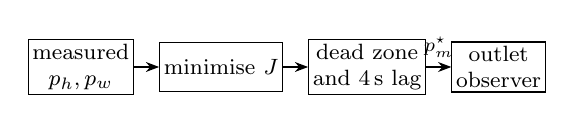
\begin{tikzpicture}[>=Stealth, font=\footnotesize, node distance=3.2mm,
  blk/.style={draw, minimum height=6.2mm, inner sep=1.5pt, align=center}]
  \node[blk] (sup) {measured\\$p_h,p_w$};
  \node[blk, right=of sup] (cost) {minimise $J$};
  \node[blk, right=of cost] (lag) {dead zone\\and \SI{4}{s} lag};
  \node[blk, right=of lag] (adrc) {outlet\\observer};
  \draw[->] (sup) -- (cost);
  \draw[->] (cost) -- (lag);
  \draw[->] (lag) -- node[above, font=\scriptsize]{$p_m^\star$} (adrc);
\end{tikzpicture}
\caption{The outlet path. The setpoint is the header pressure that keeps the inlet stems near their design openings.}
\label{fig:auth}
\end{figure}

\section{A soft sensor whose bias can be removed}
At the mix point the original extract predicted from the design mother-beer extract $P_h^\circ=16\degP$ and the filtered flows is
\begin{equation}
\label{eq:soft}
\hat{P}=\frac{\rho_h Q_h P_h^\circ}{\rho_h Q_h+\rho_w Q_w}.
\end{equation}
It is available every sample. It does not know that the true mother beer may have moved. The analyser is a delay $\tau_d=L/v_b$, limited to $[3,30]$ seconds, followed by a lag $T_a=\SI{1.2}{s}$. The delay is a shift register indexed by the current speed. At the design speed $\tau_d=\SI{9.87}{s}$. At \SI{12.91}{\cubic\metre\per\hour} in the \SI{50}{mm} outlet it falls to \SI{7.67}{s}.

The bias that reconciles $\hat{P}$ with the analyser is
\begin{equation}
\label{eq:bias}
\dot{b}_P=\frac{1}{T_b}\Big(P_{\mathrm{meas}}(t)-\hat{P}(t-\tau_d-T_a)-b_P\Big),
\end{equation}
with $T_b=\SI{28}{s}$ and $b_P$ limited to $\pm 1.5\degP$. The extract controller sees $P_c=\hat{P}+b_P$, not the raw analyser. The equilibrium of \eqref{eq:bias} is $b_P=P-\hat{P}$ when the signals are constant. Subtracting $b_P$ inside the innovation is the whole of the consistency argument. An update that uses $P_{\mathrm{meas}}-\hat{P}(t-\tau_d)$ and does not subtract $b_P$ is not observable. If a transient has left $b_P$ at $0.2\degP$, the controller drives $\hat{P}$ to the setpoint minus $0.2$, the analyser then agrees with the delayed soft sensor, and the innovation is zero. The beer stays $0.2\degP$ light forever. Subtracting $b_P$ makes that situation an innovation of $-0.2\degP$, and the bias returns to zero. When the mother beer really has changed, $P-\hat{P}$ remains and $b_P$ converges to it. This is the same consistency condition as the model-error channel of a Smith predictor \cite{smith1957closer,zheng2014predictive,zhao2014delay}.

The extract loop itself is a first-order active disturbance rejection controller on the ratio $R$. At the design ratio $\partial P/\partial R=-8.884\degP$, the design model has time constant \SI{2.2}{s}, and $b_{0,R}=-8.884/2.2=-4.038$. The coefficient is recomputed from the current ratio, so at the sales brand \SI{11.2}{\plato}, where $R=0.434$ and $\partial P/\partial R=-7.74\degP$, it moves to about $-3.52$. The bandwidths are $\omega_{c,R}=0.12$ and $\omega_{o,R}=0.48$, seven times slower than the flow loops and about twice as fast as the analyser-only baseline, which must stay at $0.055$ and $0.22$ to remain stable. The extra speed exists only because $P_c$ is not delayed. With the ratio held fixed, a hidden rise of the mother beer from $16.0$ to \SI{16.6}{\plato} is an extract change of $(11.2/16)\times 0.6=0.42\degP$ at the mix point. Equation~\eqref{eq:soft} does not contain it. Equation~\eqref{eq:bias} is the only path by which it enters $P_c$.

\section{Evidence from the joint campaign}
The coordinator and the soft sensor are estimated together with the installed-gain inlet loops of the companion paper. The baselines are ratio proportional--integral control and fixed-gain active disturbance rejection, both with the header setpoint frozen at \SI{2.40}{\barg} and with extract feedback taken from the analyser. Table~\ref{tab:win} gives the integrals on the windows that belong to this paper.

\begin{table}[!t]
\caption{Extract IAE ($\degP\cdot\mathrm{s}$) and beer-flow IAE. PID and LADRC hold the header at \SI{2.40}{\barg}.}
\label{tab:win}
\centering
\footnotesize
\begin{tabular}{@{}lrrrrrr@{}}
\toprule
 & \multicolumn{3}{c}{Extract} & \multicolumn{3}{c}{Beer flow} \\
\cmidrule(lr){2-4}\cmidrule(lr){5-7}
Window & PID & LADRC & Prop. & PID & LADRC & Prop. \\
\midrule
Brand & 76.2 & 39.6 & 19.2 & 8.73 & 11.3 & 5.08 \\
Rate & 77.3 & 6.25 & 3.68 & 74.9 & 69.3 & 4.83 \\
Drift & 147 & 18.0 & 17.4 & 65.8 & 73.9 & 3.99 \\
Wear & 216 & 7.22 & 6.05 & 121 & 135 & 4.60 \\
\bottomrule
\end{tabular}
\end{table}

On the brand change, from \SI{12.0}{\plato} to \SI{11.2}{\plato} in \SI{25}{s}, the proposed extract integral is half the analyser-based observer and a quarter of the proportional--integral loop. The proposed loop re-enters $\pm 0.05\degP$ about \SI{64}{s} after the ramp ends. Neither baseline has settled when the throughput ramp begins. The peak proposed error during the ramp is \SI{0.51}{\plato}, which is the cost of keeping the extract loop slower than the flow loops.

On the throughput window the beer-flow integrals separate the coordinator from a composition loop that is allowed to abandon the rate. Both baselines reach a beer stem near $0.98$ and stay there. At \SI{360}{s} the fixed-gain observer holds the extract at \SI{11.16}{\plato} against a setpoint of \SI{11.20}{\plato}, while the beer flow is \SI{7.96}{\cubic\metre\per\hour} against \SI{9}{\cubic\metre\per\hour}. The proposed beer flow at the same instant is \SI{8.90}{\cubic\metre\per\hour}, the header is near \SI{1.45}{\barg}, and the three stems are near $0.70$. The extra outlet travel of the full run, $3.44$ against $1.41$ and $0.61$, is this motion. It is three slow moves, at the supply step, at the throughput ramp and at the loss of $K_v$, not a chatter band.

On the hidden drift of the mother beer the two observer-based extract integrals are close, $18.0$ and $17.4$, because both eventually see the analyser. The proposed beer-flow integral on that window remains $3.99$, against $73.9$, because the drift trim does not have to be performed with the beer valve already on the stop. At \SI{520}{s} the proposed extract is \SI{11.33}{\plato} against \SI{11.20}{\plato}. The residual is the \SI{28}{s} bias lag still finishing, not a frozen offset. A shorter bias time reduces the residual and, on this plant, overshoots the setpoint.

\section{Bandwidth order, and the windows that test it}

The four bandwidths are an order, not four independent tunings. Inlet flow loops run at $\omega_c=0.85$ and $\omega_o=2.5$. The header base values are $0.20$ and $0.80$, with a scheduled ceiling of $0.44$ and $1.6$. The extract loop on $P_c$ runs at $0.12$ and $0.48$. The analyser-only baseline is held at $0.055$ and $0.22$, the highest pair that stays stable when the feedback is the raw measurement. The inequalities $\omega_{c,R}<\omega_{c,p}<\omega_{c,\mathrm{flow}}$ are the design. They were not the first values tried. A header observer at $\omega_{c,p}=0.55$, close to the flow loops, is stable on a unit-gain test and unstable on the sticky valve: the first slip grows into a cycle of period about \SI{4}{s}, with the header swinging by several tenths of a bar, before any external disturbance is applied. Slowing the header loop and ignoring setpoint changes inside \SI{0.04}{\barg} removes the cycle. The same plant then holds the design extract for a \SI{50}{s} noise-only interval with zero valve travel.

The supply step and the water oscillation are the windows in which this separation is visible before the throughput ramp spends the stroke. From \SI{50}{s} to \SI{130}{s} the extract integrals are $4.03$, $5.53$ and $3.36\degP\cdot\mathrm{s}$. Settling to $\pm 0.05\degP$ takes \SI{72}{s} for proportional--integral control and \SI{46}{s} for the coordinated controller. The frozen-gain observer does not stay inside the band. The proposed header leaves \SI{2.40}{\barg} within a few seconds and settles near \SI{1.8}{\barg}, and the beer stem opens only to about $0.68$. Both baselines hold \SI{2.40}{\barg}, and the proportional--integral beer stem reaches $0.91$. Outlet travel on the window is $1.02$ against $0.41$ and $0.12$. That travel is the coordinator buying back the drop.

From \SI{130}{s} to \SI{210}{s} the water supply oscillates with amplitude \SI{0.28}{\barg} and period \SI{26}{s}. Peak extract errors are $0.109$, $0.140$ and $0.086\degP$. Time spent outside $\pm 0.05\degP$ is \SI{30}{s}, \SI{32}{s} and \SI{7.8}{s}. The oscillation enters the water-valve gain on the sample it occurs, lagged into $b_0$ by the \SI{2.5}{s} gain filter of the companion paper. The header loop moves as well, because the cost \eqref{eq:J} sees a changing water supply, but the outlet motion is a slow modulation of travel $0.55$ on the window, not a copy of the \SI{26}{s} sine. The dead zone and the \SI{4}{s} lag are what keep it slow.

The high-rate stems can be checked without the closed loop. After the brand change, $R=(\rho_h/\rho_w)(16.0/11.2-1)=0.434$. A beer flow of \SI{9.00}{\cubic\metre\per\hour} then asks for \SI{3.91}{\cubic\metre\per\hour} of water and \SI{12.91}{\cubic\metre\per\hour} at the outlet. At a header of \SI{1.45}{\barg} and a beer supply of \SI{3.05}{\barg} the drops are \SI{1.60}{\barg}, \SI{2.75}{\barg} and \SI{0.90}{\barg}, and \eqref{eq:stem} returns stems $0.70$, $0.69$ and $0.70$. All three lie in the window where \eqref{eq:alpha} leaves the header bandwidth at its base value. The same flows at a frozen header of \SI{2.40}{\barg} ask the beer valve for a stem above one. The closed loop of the campaign settles on this static picture: at \SI{360}{s} the proposed stems are near $0.70$ and the beer flow is \SI{8.90}{\cubic\metre\per\hour}.

One further consistency check belongs to the bias. At the sales brand the sensitivity of blend extract to mother-beer extract is $P/P_h=11.2/16=0.700$. The hidden rise of $0.6\degP$ is therefore $0.42\degP$ at the mix point if the ratio is not yet trimmed. A bias time of \SI{28}{s} is about three times the design delay. It is slow enough not to overshoot and fast enough that the residual at \SI{520}{s}, \SI{0.13}{\plato}, is still closing. The proportional--integral loop, already on the beer-valve stop, finishes the drift window near \SI{13.3}{\plato}. An extract specification that ignored the production rate would rank the frozen-gain observer, which ends the campaign at \SI{11.16}{\plato} and \SI{7.38}{\cubic\metre\per\hour}, ahead of a controller that is still closing a \SI{0.13}{\plato} residual at the demanded rate. A blending specification ranks them the other way.

\section{Full-run balance of error and travel}
Table~\ref{tab:full} is the \SI{560}{s} integral, not a selected window. The proposed extract integral is $64$ percent of the frozen-gain observer and about one tenth of the proportional--integral loop. The beer-flow integral is about one eighth of either baseline. Dividing by the length of the run, the proposed mean absolute errors are $52.4/560=0.094\degP$ and $37.5/560=0.067\,\mathrm{m}^3\mathrm{h}^{-1}$. The frozen-gain means are $0.145\degP$ and $0.57\,\mathrm{m}^3\mathrm{h}^{-1}$. The proportional--integral means are $0.94\degP$ and $0.51\,\mathrm{m}^3\mathrm{h}^{-1}$. The two baseline flow means are similar because both lose the beer valve for the same physical reason, a header that was not allowed to fall. Their extract means differ because the observer still trims water from the analyser, while the proportional--integral loop, once the beer flow is stuck, trims water from a ratio that no longer describes the plant.

\begin{table}[!t]
\caption{Full-run indices, \SIrange{0}{560}{s}. Travel is the integrated absolute stem speed.}
\label{tab:full}
\centering
\begin{tabular}{@{}lrrr@{}}
\toprule
Index & PID & LADRC & Prop. \\
\midrule
Extract IAE ($\degP\cdot\mathrm{s}$) & 524 & 81.4 & 52.4 \\
Beer-flow IAE & 286 & 316 & 37.5 \\
Time outside $\pm 0.05\degP$ (s) & 384 & 333 & 271 \\
Beer-valve travel & 2.99 & 5.93 & 7.02 \\
Water-valve travel & 2.33 & 3.86 & 5.14 \\
Outlet-valve travel & 0.61 & 1.41 & 3.44 \\
\bottomrule
\end{tabular}
\end{table}

The steady window before the supply step is the noise floor. All three controllers integrate about $0.005\degP\cdot\mathrm{s}$ of extract error and $0.007\,\mathrm{m}^3\mathrm{h}^{-1}\mathrm{s}$ of flow error, and the valve travel on that interval is zero. The extra travel in Table~\ref{tab:full} is therefore not a loop that chatters inside the stick band. It is the outlet stroke spent at the supply step, at the throughput ramp and at the loss of $K_v$. A quiet loop that finishes at the wrong flow is not the better design \cite{bialkowski1993dreams,hagglund1995monitor}. The first \SI{50}{s} are the check that the dead zone, the \SI{4}{s} lag and the base header bandwidth really do leave a sticky valve alone when nothing has happened.

The same table is not a flavour result. A correct original extract does not restore the foam and ester differences that high-gravity fermentation itself introduces \cite{stewart2010highgravity,briggs2004brewing}. The coordinator and the soft sensor keep the extract and the flow at the values the brand and the production plan specify. They do not enlarge the set of mother beers the brewery can ferment, and they do not remove the need for the installed-gain inlet loops of the companion paper. A correct header setpoint with a wrong $b_0$ still mis-scales the flow command. A correct soft sensor with the beer valve on the stop still cannot deliver the rate.

\section{One sample, in order}
The controller is a fixed sequence at $\Delta t=\SI{10}{ms}$, which is the sequence a function block would execute. Read the filtered flows, stems and pressures. Compute $\tau_d=L/v_b$ and take the shift-register index nearest $\tau_d/\Delta t$. At the design speed that index is $987$ samples; at \SI{12.91}{\cubic\metre\per\hour} it is $767$ samples. Update $b_P$ from \eqref{eq:bias} using the soft sensor delayed by $\tau_d+T_a$, not by $\tau_d$ alone, because the analyser lag shifts the measurement as well as smoothing it. Step the extract observer and form $Q_w^\star=R Q_h^\star$. Step the two inlet observers of the companion paper. Evaluate $J$ on the hundred-point grid, pass the minimiser through the \SI{0.04}{\barg} dead zone and the \SI{4}{s} setpoint lag, update $\alpha$ from \eqref{eq:alpha}, and step the header observer. Lag the three stem commands by \SI{0.40}{s} and return those lagged commands both to the positioners and to the observers as the applied input of the next sample.

The extract loop is stepped before the flow loops so that the water setpoint of this sample already contains the latest ratio. The header loop is stepped after the inlet commands so that it sees their effect through the plant, one sample later. A one-sample delay at \SI{10}{ms} is negligible beside a \SI{2.4}{s} positioner. Closing the algebraic loops inside one sample, by iterating the observers to convergence, changed nothing measurable.

During the \SI{20}{s} throughput ramp the index $L/v_b(t)$ is not identical to the travel time of the fluid element now leaving the pipe, because that element entered when the speed was lower. The difference is a fraction of a second. Beside $T_a=\SI{1.2}{s}$ and $T_b=\SI{28}{s}$ it does not move the innovation enough to justify integrating $1/v$ along the pipe. After the ramp settles, current speed and travel time coincide, and the index is exact.

The proportional--integral baseline that this sequence is compared with is a velocity form with the same command limits and the same stick model. Its beer gain is $0.272$ with integral time \SI{2.4}{s}, its water gain is $0.516$ with the same integral time, its header gain is $0.150$ with integral time \SI{8}{s} and a setpoint fixed at \SI{2.40}{\barg}, and its extract gain on the ratio is $-0.0088$ with integral time \SI{22}{s}. The header gain is positive: a high header opens the outlet. The extract gain is negative because $\partial P/\partial R<0$. The frozen-gain observer uses the flow and header bandwidths of the proposed controller and differs in the three places this paper and its companion name: frozen $b_0$, fixed header setpoint, analyser feedback. Retuning those baselines on the disturbed plant would compare tuning effort, which is a different question.

\section{Conclusion}
Loss of valve authority and analyser delay are separate faults, and they need separate signals. The outlet valve, driven to a header setpoint that minimises a stem cost, returns the pressure drop the inlet valves lose when a supply falls. The mass-balance soft sensor lets the extract loop run at a cascade bandwidth, and the delayed analyser corrects only a bias, provided the bias is subtracted inside its own innovation. Together with the installed-gain inlet loops of the companion paper, the pair keeps a beer flow of \SI{9}{\cubic\metre\per\hour} inside the stroke at a beer supply of \SI{3.05}{\barg} and brings a brand change back to the tolerance band before either analyser-based baseline has settled. The outlet travel is the price of the first result, and the bias lag is the price of the second.

\bibliographystyle{IEEEtran}
\bibliography{refs}

\end{document}
